% This is part of Un soupçon de mathématique sans être agressif pour autant
% Copyright (c) 2015
%   Laurent Claessens
% See the file fdl-1.3.txt for copying conditions.

\begin{exercice}[\cite{NRHooXFvgpp5}]\label{exo2smath-0098}

Les droites \( (TR)\) et \( (LU)\) sont parallèles et \( \widehat{REA}=\SI{60}{\degree}\). Lesquelles des proposition suivantes sont vraies ?

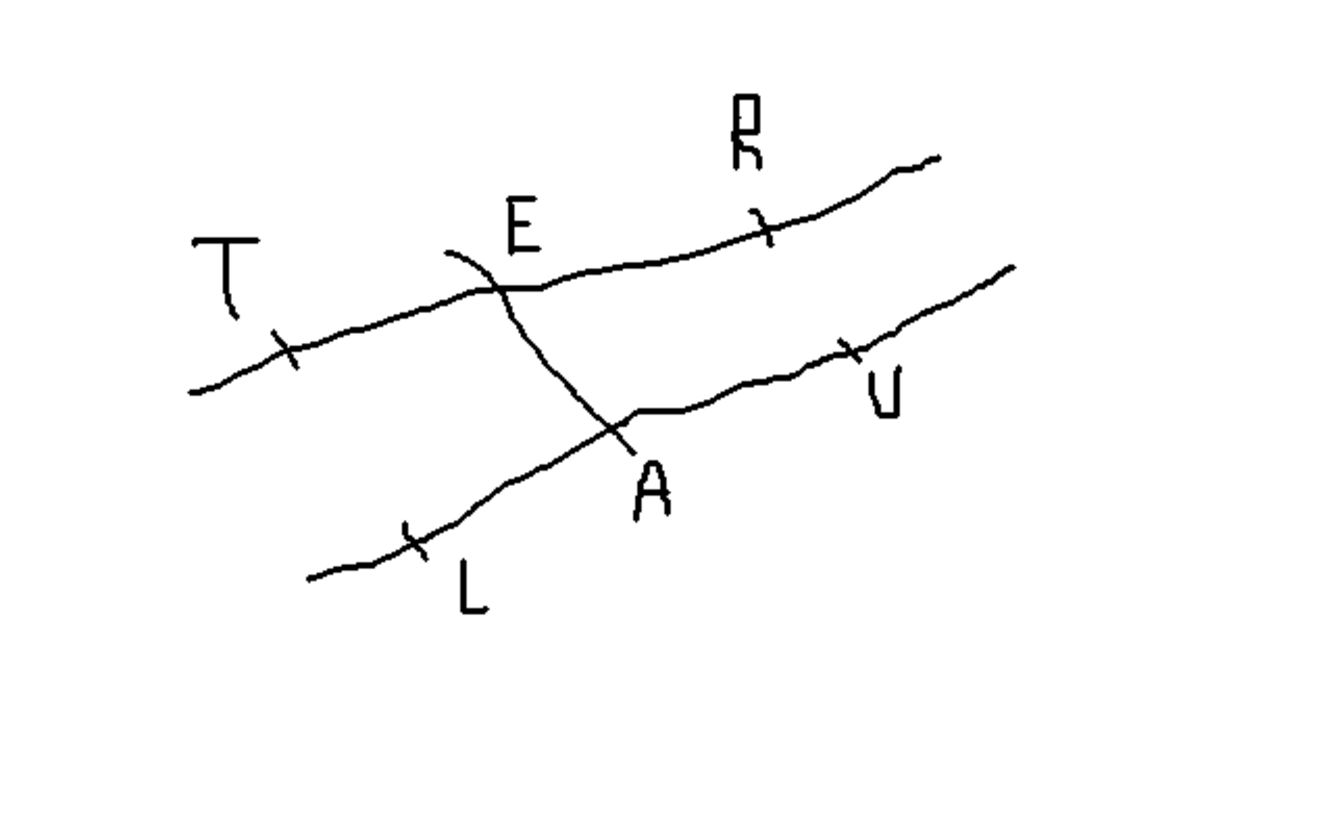
\includegraphics[width=5cm]{faux_angles.pdf}

\begin{multicols}{2}
\begin{enumerate}
    \item
        \( \widehat{EAL}=\SI{60}{\degree}\)
    \item
        \( \widehat{TEA}=\SI{120}{\degree}\)
    \item
        \( \widehat{EAU}=\SI{60}{\degree}\)
    \item
        \( \widehat{EAU}=\SI{120}{\degree}\)
\end{enumerate}
\end{multicols}

\corrref{2smath-0098}
\end{exercice}
